% !TEX root = main.tex
%\myparagraph{Key points}
%\begin{enumerate}[1.]
%%	\item	Session $\pi$ calculus with process passing. DONE
%%	\item	Identify session $\pi$ and process passing subcalculi and their polyadic variants. DONE
%%	\item	Bisimulation theory for higher-order session semantics. DONE
%%	\item	New triggered bisimulation, related to J\&R's. DONE
%%	\item   Elementary values key to characterizations of behavioural equivalence. DONE
%	\item	Types provide techniques to prove completeness without matching. \jp{TBD}
%	\item	We are interested in encodings with properties a la Gorla. 
%                We extended them to typed setting. \jp{TBD}
%%	\item	Encode name-passing to pure process abstraction calculus, with name abstractions. DONE
%%	\item	Type of the recursion encoding uses non tail recursive type $\trec{t}{\btinp{t} \tinact}$. DONE
%%	\item	Encode higher-order semantics to first order semantics. DONE
%%	\item	Negative result. Cannot encode shared names using only shared names.
%%	\item   Extensions with higher-order abstractions and polyadicity also explored. DONE
%\end{enumerate}

%\smallskip 
%
%\myparagraph{Important things to explain}
%Explain our \HO is very small without containg name passing 
%\[ 
%\abs{x}.P \quad \appl{x}{u}
%\]

%Explain we input only characteristic processes.  
%
%\[
%\lambda x.\mapchar{S}{x}
%\]

%\subsection{Higher-Order Session Calculi}
\noi 
By combining features from the $\lambda$-calculus and the $\pi$-calculus, 
in \emph{higher-order process calculi} exchanged values may contain  processes. 
In this paper, we consider higher-order calculi with \emph{session primitives},
thus enabling the specification of reciprocal exchanges (protocols) 
for higher-order mobile processes, 
which can be verified via type-checking using \emph{session types}~\cite{honda.vasconcelos.kubo:language-primitives}.
%These calculi allow us to specify   
%session protocols in which higher-order values 
%(mobile code) can be exchanged in a type-safe manner. 
%; 
%governed by session types, 
%such protocols cleanly distinguish between 
%linear and unrestricted behaviors in 
%%directed %point-to-point 
%communications.
The study of higher-order concurrency has received significant attention, 
from untyped and typed perspectives (see, e.g.,~\cite{ThomsenB:plachoasgcfhop,SangiorgiD:expmpa,San96int,JeffreyR05,MostrousY15,DBLP:journals/iandc/LanesePSS11,DBLP:conf/icalp/LanesePSS10,DBLP:conf/esop/KoutavasH11,XuActa2012}).
%in particular via  comparisons with the first-order mobility of the $\pi$-calculus~\cite{MilnerR:calmp1}. 
Although models of session-typed 
communication with features of higher-order concurrency exist~\cite{tlca07,DBLP:journals/jfp/GayV10},
their  \emph{tractable behavioural equivalences} and \emph{relative expressiveness}
remain little understood. 
%for higher-order session calculi. 
%these two issues 
%have been throughly studied
%%are well-understood 
%for higher-order languages without sessions \cite{},
%but not for higher-order process calculi with sessions.
%This is unfortunate, given the wide applicability of session-based concurrency; indeed,
%session types are expressive enough to describe complex 
%communication structures found in practical protocols,  expressible, e.g., via recursive session types.
%Clarifying the status of typed equivalences and relative expressiveness for session languages
Clarifying their status is not only useful for, 
e.g.,~justifying non-trivial mobile protocol
optimisations, but also for transferring key reasoning techniques
between (higher-order) session calculi. Our discovery 
is that \emph{linearity} of session types plays a vital role to 
offer new equalities and fully abstract encodability, 
which to our best knowledge have not been proposed before.   

The main higher-order language in our work, denoted \HOp,
extends the higher-order $\pi$-calculus~\cite{SangiorgiD:expmpa} with session primitives:
it contains constructs for 
%session establishment
synchronisation on shared names, 
recursion, 
name abstractions (i.e., functions from name identifiers  to processes, 
\jpc{denoted}
$\lambda x.P$) and applications 
\jpc{(denoted $(\lambda x.P)a$)};
and session communication (value passing and
labelled choice using linear names). 
We study two significant subcalculi of \HOp, 
\jpc{which}
distil higher- and first-order mobility:
the \HO-calculus, which is \HOp without recursion and name passing, and 
the session \sessp-calculus \jpc{(here denoted~\sessp)}, which is \HOp without abstractions and applications.  
While \sessp is, 
in essence, the calculus in~\cite{honda.vasconcelos.kubo:language-primitives}, 
this paper shows that \HO  is a new core calculus 
for higher-order session concurrency.

In the first part of the paper, we address tractable behavioural equivalences
for \HOp.
A well-studied behavioural equivalence in the higher-order setting 
is \emph{context bisimilarity}~\cite{San96H},
a labelled characterisation of reduction-closed, barbed congruence, 
which offers an appropriate discriminative power at the price of heavy universal quantifications in output clauses.
Obtaining alternative characterisations 
is thus a recurring issue 
in the study of higher-order calculi. 
Our approach 
shows that protocol specifications given by session types are 
essential to  limit 
the behaviour of higher-order session processes. 
Exploiting elementary processes inhabiting session types, 
this limitation is formally enforced by 
a refined (typed) labelled transition system (LTS)
that narrows down the spectrum of allowed process behaviours, 
thus enabling tractable reasoning techniques. 
Two tractable characterisations of bisimilarity 
are then introduced. 
%shown to coincide with context bisimilarity.
Remarkably, using session types we prove that these %tractable
bisimilarities coincide with context bisimilarity, without using
operators for 
name-matching.
%Remarkably session type structures enable to provide 
%a coincidence without name-matching operators in the calculi.

We then move on to 
%in the second part of the paper we 
assess the expressivity 
 of \HOp, \HO, and \sessp as delineated by typing. 
We establish strong correspondences between 
these calculi  via type-preserving, fully abstract encodings up to 
behavioural equalities. While encoding \HOp 
into the $\pi$-calculus preserving session types 
(extending  known  results for untyped processes) is 
%\jpc{already}
significant, 
our main contribution is 
an encoding of \HOp into \HO, where name-passing is absent.  

We illustrate the essence of encoding name passing into \HO: 
to encode name output, we ``pack''
the name to be passed around into a suitable abstraction; 
upon reception, the receiver must ``unpack'' this object following a precise protocol.
More precisely, our encoding 
\jpc{of name passing}
in \HO is given as:
\begin{center}
\begin{tabular}{rcll}
  $\map{\bout{a}{b} P}$	&$=$&	$\bout{a}{ \abs{z}{\,\binp{z}{x} (\appl{x}{b})} } \map{P}$ \\
  $\map{\binp{a}{x} Q}$	&$=$&	$\binp{a}{y} \newsp{s}{\appl{y}{s} \Par \bout{\dual{s}}{\abs{x}{\map{Q}}} \inact}$
\end{tabular}
\end{center}
\noi where $a,b$ are names; $s$ and $\dual{s}$ are 
linear names (called \emph{session endpoints});
%$\lambda x.P$ is a name abstraction of $P$; $\appl{x}{a}$ is a name application; 
$\bout{a}{V} P$ and 
$\binp{a}{x} P$ denote an output and input at~$a$;   
and $\newsp{s}P$ is hiding. 
A (deterministic) reduction between   endpoints 
$s$ and $\dual{s}$ guarantees name $b$ is properly unpacked.
Encoding a recursive process $\recp{X}{P}$ is \NY{also} challenging, for 
the linearity of endpoints in $P$ must be preserved.
We encode recursion with non-tail recursive session types; for this 
we apply recent advances on the theory of session duality~\cite{TGC14,DBLP:journals/corr/abs-1202-2086}.
%\dk{Encoding of a general recursive process $\recp{X}{P}$ is another challenge, since 
%it must preserve the linearity of session endpoints appeared in $P$.
%We encode it with non-tail recursive session types,  
%for which we apply a recent advance on a session duality theory 
%\cite{BernardiH14,TGC14,DBLP:journals/corr/abs-1202-2086}.}

We further extend our encodability results to 
i)~\HOp with \emph{higher-order} abstractions (denoted \HOpp) 
and to ii)~\HOp with polyadic name passing and abstraction (\pHOp); and to
their super-calculus  (\PHOpp) (equivalent to the calculus in~\cite{tlca07}). 
%Here again the usage information given by session types is essential to define encodings
%and to state their semantic correspondences.
% Building upon established notions for (untyped) processes~(e.g.,~\cite{DBLP:journals/iandc/Gorla10}), 
% we
%define a notion of \emph{precise encoding} that 
%requires the translation of both process and types, and 
%focuses on process mappings that preserve (session) typing. 
%Thus, our encodings only relate source and target 
%processes 
%with  
%proper communication structures (given by session types).
A further result shows that 
shared names
%as required in the session establishment phase,
strictly add expressive power 
to session calculi. 
\figref{fig:express} summarises %our expressivity 
these results. %including the three extensions of \HOp. 

\begin{figure}[t]
\centering
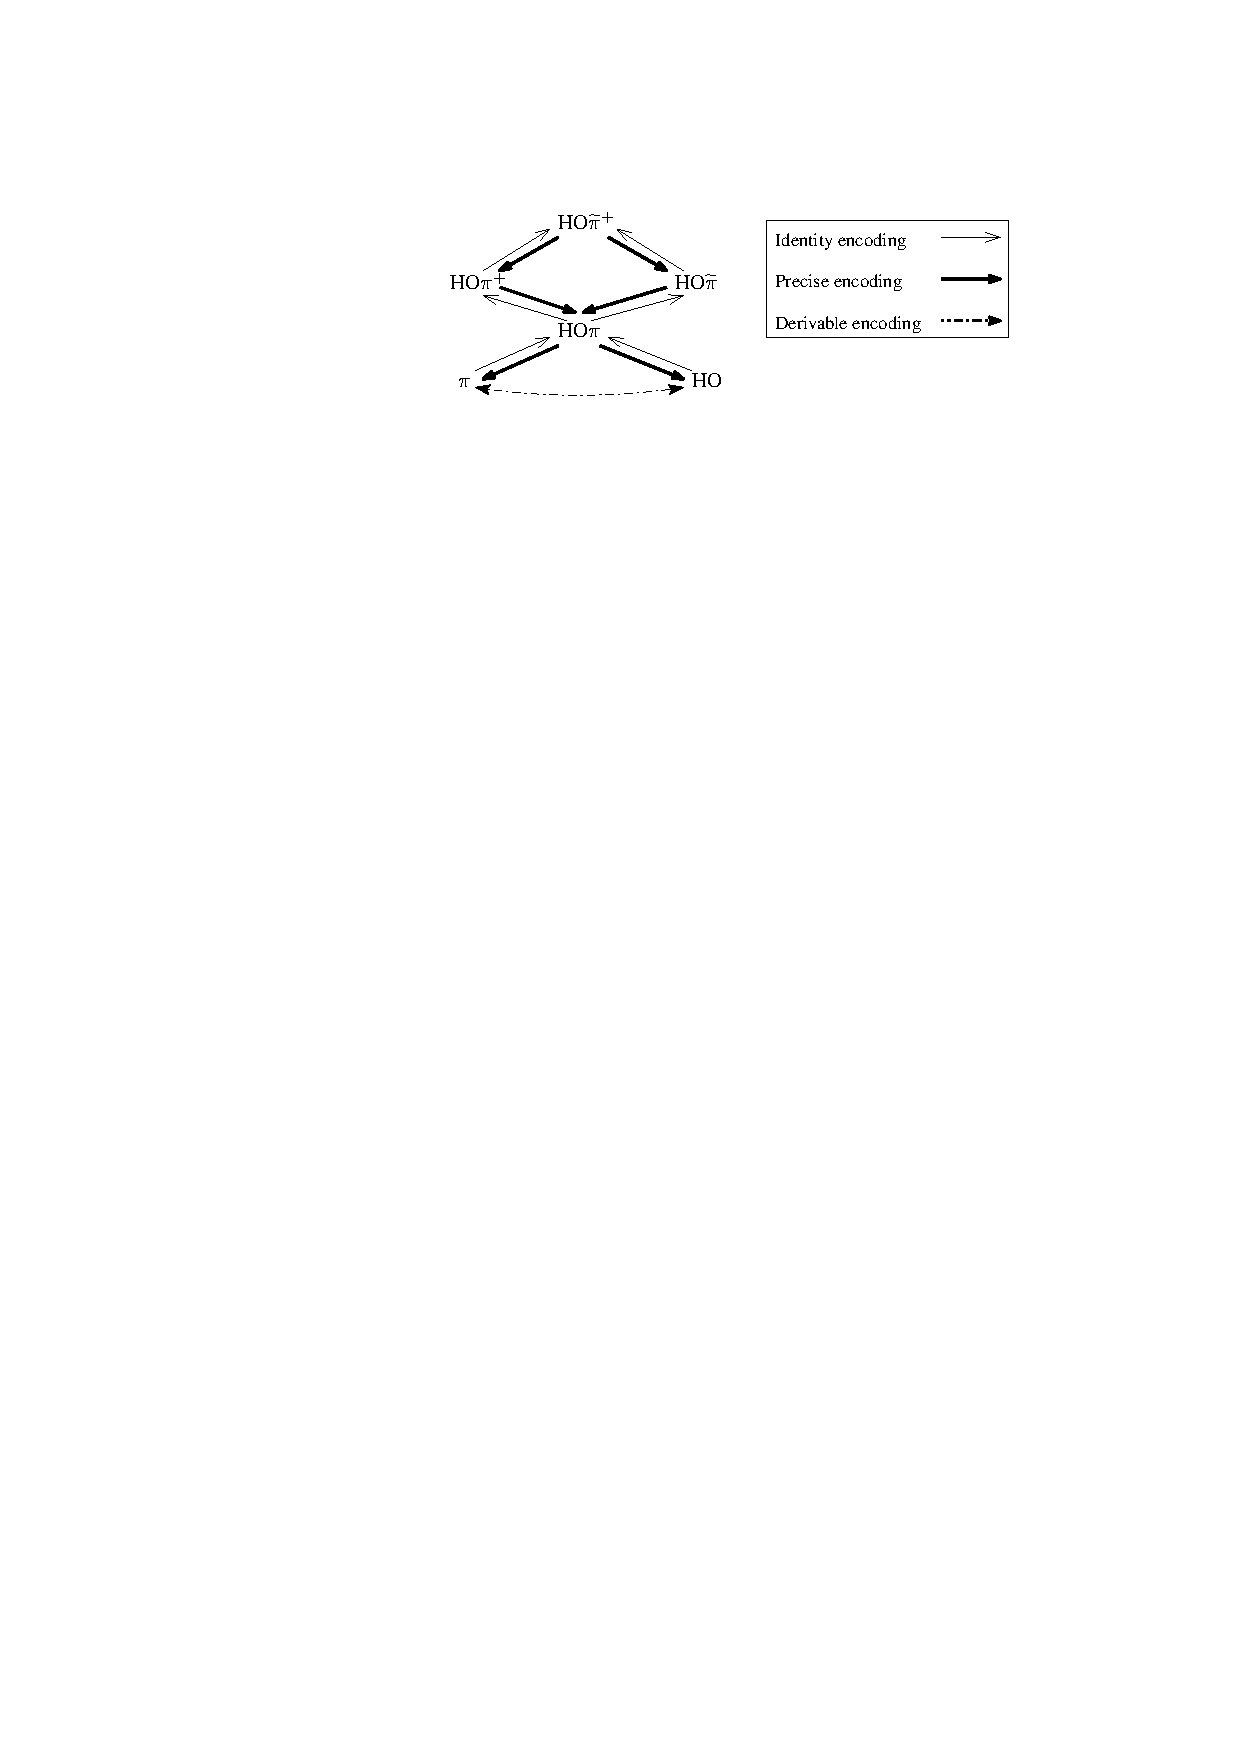
\includegraphics[scale=1]{diag.pdf}
\vspace{1mm}
%%ADD~FIGURE!
%	\centering
%	\begin{subfigure}[b]{0.45\linewidth}
%		\centering
%		\begin{tikzpicture}
%
%			\node	(PHOpp)	at	(0, 0.8)		{\PHOpp};
%			\node	(HOpp)	at	(-1.5, 0.4)	{\HOpp};
%			\node	(PHOp)	at	(1.5, 0.4)	{\PHOp};
%			\node	(HOp)	at	(0, 0)		{$\mathsf{HO}{\pi}^{~}$};
%			\node	(HO)	at	(-1.5, -0.4)	{$\mathsf{HO}{~}^{~}$};
%			\node	(sessp)	at	(1.5, -0.4)	{$~~\pi^{~}$};
%
%			\draw[<-]	(PHOpp) -- (HOpp);	%(0, 1.25) -- (-2, 1);
%			\draw[<-]	(PHOpp) -- (PHOp);	%(0, 1.25) -- (2, 1);
%
%			\draw[<-]	(HOpp) -- (HOp);	%(2, 0.5) -- (0, 0.25);
%			\draw[<-]	(PHOp) -- (HOp);	%(-2, 0.5) -- (0, 0.25);
%
%			\draw[<-]	(HOp) -- (HO);		%(0, -0.25) -- (-2, -0.5);
%			\draw[<-]	(HOp) -- (sessp);	%(0, -0.25) -- (2, -0.5);
%
%%				\node	(PHOpp)	at	(0, 0.8)		{\PHOpp};
%%				\node	(HOpp)	at	(-2, 0.4)	{\HOpp};
%%				\node	(PHOp)	at	(2, 0.4)	{\PHOp};
%%				\node	(HOp)	at	(0, 0)		{$\mathsf{HO}{\pi}^{~}$};
%%				\node	(HO)	at	(-2, -0.4)	{$\mathsf{HO}{~}^{~}$};
%%				\node	(sessp)	at	(2, -0.4)	{$~~\pi^{~}$};
%%
%%				\draw[->]	(PHOpp) -- (HOpp);	%(0, 1.25) -- (-2, 1);
%%				\draw[->]	(PHOpp) -- (PHOp);	%(0, 1.25) -- (2, 1);
%%
%%				\draw[->]	(HOpp) -- (HOp);	%(2, 0.5) -- (0, 0.25);
%%				\draw[->]	(PHOp) -- (HOp);	%(-2, 0.5) -- (0, 0.25);
%%
%%				\draw[->]	(HOp) -- (HO);		%(0, -0.25) -- (-2, -0.5);
%%				\draw[->]	(HOp) -- (sessp);	%(0, -0.25) -- (2, -0.5);
%		\end{tikzpicture}
%	\end{subfigure}
%%	\hfill
%	\begin{subfigure}[b]{0.5\linewidth}
%		\small
%		The arrow start calculus wrt arrow tip calculus:
%		\begin{itemize}
%			\item	is a sub-calculus.
%			\item	encodes.
%		\end{itemize}
%		Arrow properties are transitive.
%	\end{subfigure}
%\\
	\caption{Encodability in Higher-Order Session Calculi. 
	Precise encodings are defined in \defref{def:goodenc}.
	\label{fig:express}}
\Hlinefig
\end{figure}

\smallskip

\myparagraph{Outline / Contributions.} This paper 
is structured as follows:
\begin{enumerate}[$\bullet$]
\item \secref{sec:overview} overviews key ideas of our tractable bisimulations.
\item \secref{sec:calculus} presents the higher-order session calculus \HOp and its 
subcalculi \HO and \sessp.  Then, \secref{sec:types} gives the session type system
and states type soundness for \HOp and its variants.
\item \secref{sec:behavioural} 
develops \emph{higher-order} and \emph{characteristic} bisimilarities, our two
tractable characterisations of contextual equivalence which 
alleviate the issues of context bisimilarity~\cite{San96H}. These 
relations are shown to coincide in \HOp (\thmref{the:coincidence}).
\item \secref{s:expr} defines \emph{precise (typed) encodings} by extending encodability criteria 
studied for
untyped processes~(e.g.~\cite{DBLP:journals/iandc/Gorla10,DBLP:conf/icalp/LanesePSS10}).
\item \secref{sec:positive} %and \S\,\ref{sec:negative}
gives encodings of \HOp into \HO and of \HOp into~\sessp.
These encodings 
are shown to be \emph{precise} (Thms.~\ref{f:enc:hopitoho} and~\ref{f:enc:hotopi}).
Mutual encodings between \sessp and \HO are derivable; 
all these calculi are thus equally expressive.
Exploiting determinacy and typed equivalences,
we also prove the non-encodability of shared names
into linear names (\thmref{t:negative}).

\item \secref{sec:extension} studies extensions of \HOp. We show that 
both \HOpp (the extension with higher-order applications) 
and \pHOp (the extension with polyadicity) are encodable in \HOp
(Thms.~\ref{f:enc:hopiptohopi} and \ref{f:enc:phopiptohopi}).
This connects our work 
to the existing
higher-order session calculus in~\cite{tlca07} (here denoted  $\PHOpp$).

\item \secref{sec:relwork} concludes with related works. The appendix summarises the typing system. 
\end{enumerate}
\noi
The paper is self-contained. 
{\bf\em Additional related work, more examples, omitted definitions, and  proofs 
%can be found
are 
in~\cite{KouzapasPY15}.} 

